\documentclass{article}

\usepackage{latexsym, amssymb}
\usepackage{graphicx}
\usepackage{rail}
\railoptions{-t -h}
\usepackage{listings}
\usepackage[usenames]{color} 

\relax

\begin{document}

\definecolor{yobg}{rgb}{0.9,0.9,1}
\definecolor{yotxt}{rgb}{0.01,0.01,0.52}
%%\newcommand{\farg}[1]{\textrm{\textit{#1}}}

% parameters for listings
\lstset{
	tabsize=4,
	showspaces=false,
	showstringspaces=false,
    language=C++, 
    basicstyle=\ttfamily\color{yotxt},
    numbers=none,
    stepnumber=2,
    %%frame=single,
    backgroundcolor=\color{yobg},
    captionpos=b
}

\title{Faust Quick Reference}
\author{Yann Orlarey\\Grame, Centre National de Creation Musicale}
\date{June 2008}


\railalias{recur}{$\sim$}
\railalias{lbrace}{\{}
\railalias{rbrace}{\}}
\railalias{dollar}{\$}
\railalias{mod}{\%}
\railalias{arobase}{@}
\railalias{ampersand}{\&}
\railalias{hat}{$\land$}
\railalias{kot}{'}
\railalias{pipe}{$|$}
\railalias{fdelay}{}
\railalias{backslash}{\char"5C}
\railterm{recur,lbrace,rbrace,dollar,mod,kot,arobase,ampersand,backslash,fdelay, pipe, hat}

\newcommand{\farg}[1]{\textrm{\textit{#1}}}
\newcommand{\ldbrack}{[\![ \,}
\newcommand{\rdbrack}{\, ]\!] }
\newcommand{\rdbrackC}{\rdbrack_{\mathrm{C}}\,}
\newcommand{\dbrack}[1]{\ldbrack #1 \rdbrack}
\newcommand{\semantic}[1]{\ldbrack #1 \rdbrack}
\newcommand{\dbrackC}[1]{\ldbrack #1 \rdbrackC}

\setlength{\parindent}{0pt}
\setlength{\parskip}{1ex plus 0.5ex minus 0.2ex}

\maketitle

FAUST (Functional Audio Stream) is a functional programming language for real-time signal processing and synthesis that targets high-performance signal processing applications and audio plug-ins for a variety of plateforms and standards. 

Its main caracteristics are :

\begin{itemize}


\item Programs are fully compiled, not interpreted. The compiler translates FAUST programs into equivalent C++ programs taking care of generating the most efficient code. The result can generally compete with, and sometimes even outperform, C++ code written by seasoned programmers. 

\item The generated code works at the sample level. It is therefore suited to implement low-level DSP functions like recursive filters. Moreover the code can be easily embedded. It is self-contained and doesn't depend of any DSP library or runtime system. It has a very deterministic behaviour and a constant memory footprint. 

\item The semantic of FAUST is simple and well defined. This is not just of academic interest. It allows the FAUST compiler to be \emph{semantically driven}. Instead of compiling a program literally, it compiles the mathematical function it denotes. This feature is useful for example to promote components reuse while preserving optimal perfomance.  

\item FAUST is a textual language but nevertheless block-diagram oriented. It actually combines two approaches: functional programming and algebraic block-diagrams. The key idea is to view block-diagram construction as function composition. For that, FAUST relies on a \emph{block-diagram algebra} of five composition operations.

\end{itemize}

This document is intended to provide a quick-reference to the FAUST language (version 0.9.9.6). The first section gives a full description of the syntax.



\section{Faust syntax}

This section describes the syntax of Faust. Figure \ref{fig:syntax} gives an overview of how this description is organized. 

\begin{figure}[ht!]
\centering
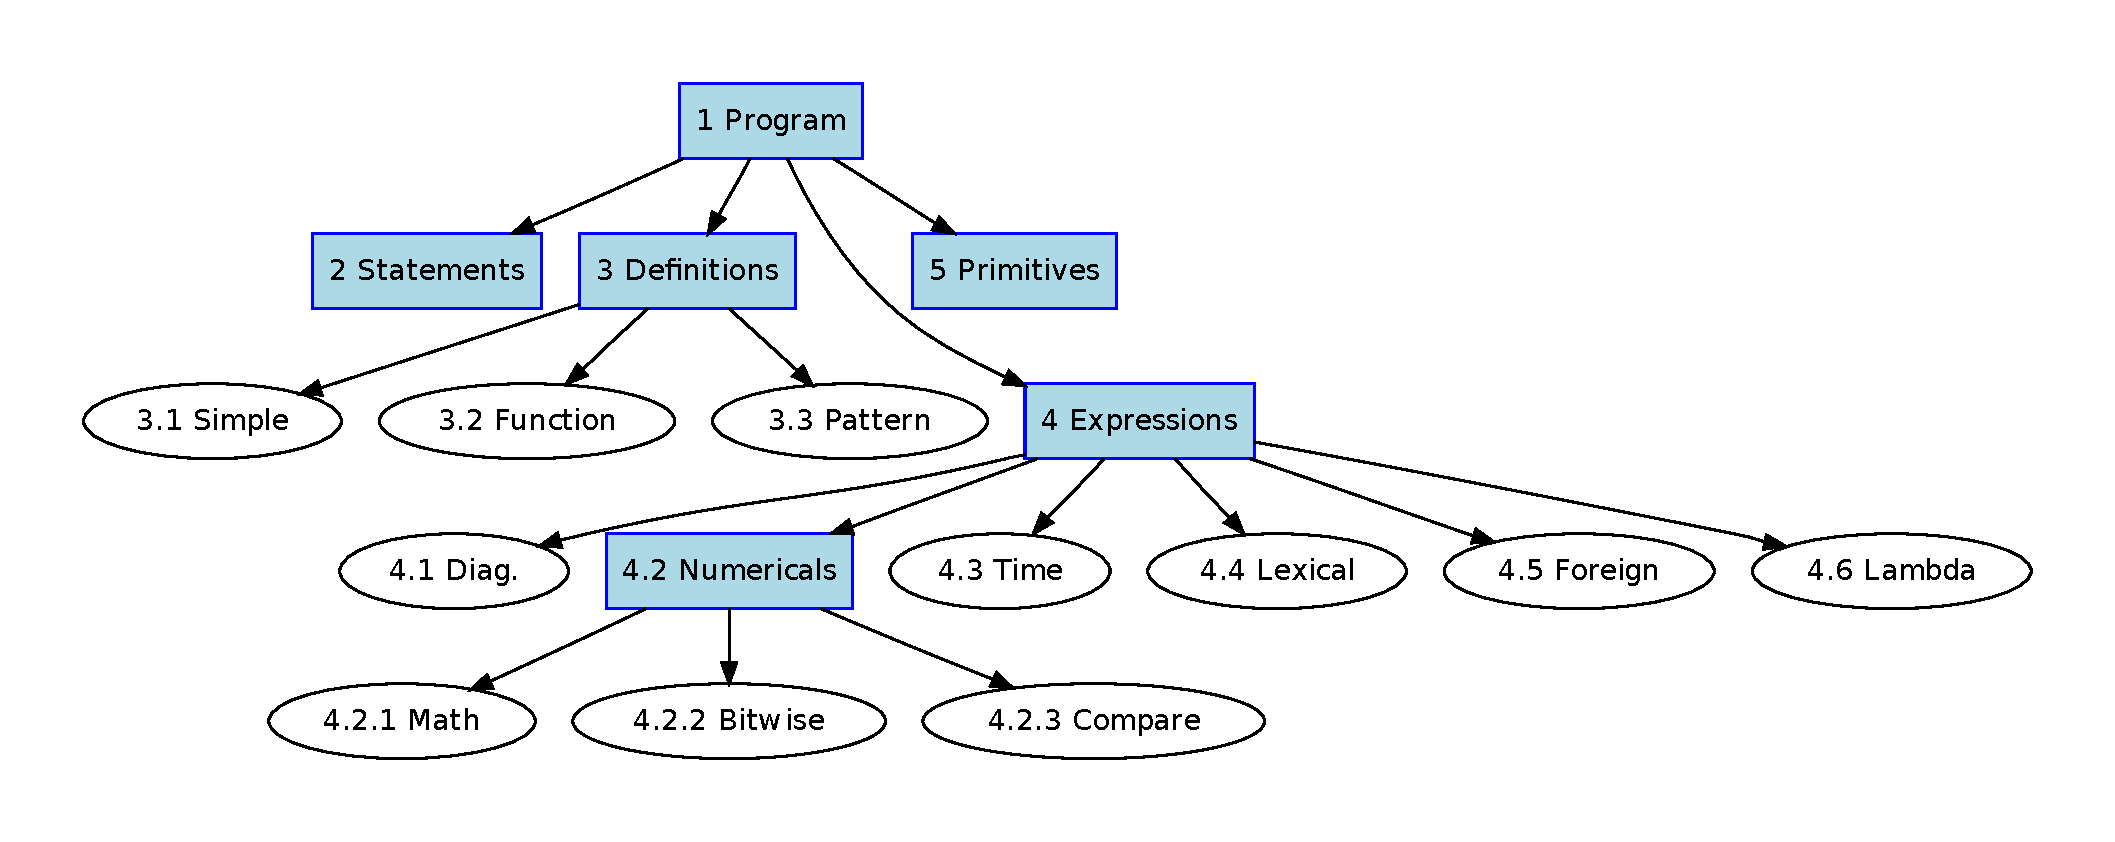
\includegraphics[scale=0.5]{illustrations/syntax-chart}
\caption{Overview of Faust syntax}
\label{fig:syntax}
\end{figure}

As we will see, \textit{definitions} and \textit{expressions} have a central role.

\subsection{Faust program}

A Faust program is essentially a list of \textit{statements}. These statements can be \textit{declarations}, \textit{imports} and \textit{definitions}, with optional C++ style (//... and /*...*/) comments.
 
\begin{rail}
program : (statement)+;
\end{rail}

Here is a short Faust program that implements of a simple noise generator. It exhibits the various kind of statements : two \textit{declarations}, an \textit{import}, a \textit{comment} and a \textit{definition}.

\begin{lstlisting}
declare name       "noise";
declare copyright  "(c)GRAME 2006";

import("music.lib");

// noise level controlled by a slider
process = noise * vslider("volume", 0, 0, 1, 0.1);
\end{lstlisting}
 
The keyword \lstinline'process' is the equivalent of \lstinline'main' in C/C++. Any FAUST program, to be valid, must at least define \lstinline'process'.

\subsection{Statements}

The \textit{statements} of a Faust program are of three kinds : \textit{metadata declarations}, \textit{file imports} and \textit{definitions}. All statements end with a semicolon (\lstinline';'). 

\begin{rail}
statement : declaration | fileimport | definition;
\end{rail}



\subsubsection{Declarations}

Meta-data declarations (for example \lstinline'declare name "noise";') are optional and typically used to document a Faust project. 

\begin{rail}
declaration : "declare" key string ';';
key : identifier;
\end{rail}

Contrary to regular comments, these declarations will appear in the C++ code generated by the compiler.

\subsubsection{Imports}

File imports allow to import definitions from other source files.  

\begin{rail}
fileimport : "import" '(' filename ')' ';';
\end{rail}

For example \lstinline{import("math.lib");} imports the definitions of the \lstinline{math.lib} library, a set of additional mathematical functions provided as foreign functions.



\subsection{Definitions}

A \textit{definition} associates an identifier with an expression it stands for. 

Definitions are essentially a convenient shortcut avoiding to type long expressions. During compilation, more precisely during the evaluation stage, identifiers are replaced by their definitions. It is therefore always equivalent to use an identifier or directly its definition. Please note that multiple definitions of a same identifier are not allowed, unless it is a pattern matching based definition.

\subsubsection{Simple Definitions}

The syntax of a simple definition is:

\begin{rail}
definition  : identifier '=' expression ';';
\end{rail} 

For example here is the definition of \lstinline'random', a simple pseudo-random number generator:

\begin{lstlisting}
 random = +(12345) ~ *(1103515245);
\end{lstlisting}


\subsubsection{Function Definition}

Definitions with formal parameters correspond to functions definitions.

\begin{rail}
definition  : identifier '(' (parameter + ',')  ')' '=' expression ';';
\end{rail} 

For example the definition of \lstinline'linear2db', a function that converts linear values to decibels, is :

\begin{lstlisting}
 linear2db(x) = 20*log10(x);
\end{lstlisting}
 
Please note that this notation is only a convenient alternative to the direct use of \textit{lambda-abstractions} (also called anonymous functions). The following is an equivalent definition of \lstinline'linear2db' using a lambda-abstraction:

\begin{lstlisting}
 linear2db = \(x).(20*log10(x));
\end{lstlisting}


\subsubsection{Definitions with pattern matching}

Moreover, formal parameters can also be full expressions representing patterns. 
\begin{rail}
definition  : identifier '(' (pattern + ',')  ')' '=' expression ';';
pattern : identifier | expression; 
\end{rail}

Let's say that you want to describe a function to duplicate an expression several times in parallel.  :
\begin{lstlisting}
 duplicate(1,exp) = exp;
 duplicate(n,exp) = exp, duplicate(n-1,exp);
\end{lstlisting}

Please note that this last definition is a convenient alternative to the more verbose :
\begin{lstlisting}
 duplicate = case { 
               (1,exp) => exp; 
               (n,exp) => duplicate(n-1,exp); 
             };
\end{lstlisting}

 
  
\subsection{Expressions}

Despite its textual syntax, Faust is conceptually a block-diagram language. Faust expressions represent DSP block-diagrams and are assembled from primitive ones using various \textit{composition} operations. More traditional \textit{numerical} expressions in infix notation are also possible. Additionally Faust provides time based expressions, like delays, expressions related to lexical environments, expressions to interface with foreign function and lambda expressions.

\begin{rail}
expression : diagram | numerical | time | lexical | foreign | lambda;
\end{rail}
  
\subsubsection{Diagram Expressions}

\paragraph{Diagram expressions} are assembled from primitive ones using either binary composition operations or high level iterative constructions.
 
\begin{rail}
diagramexp : diagcomposition | diagiteration;
\end{rail}

\paragraph{Five composition operations} are available : \textit{recursion}, \textit{parallel}, \textit{sequential}, \textit{split} and \textit{merge} composition.

\begin{rail}
diagcomposition : expression (recur|','|':'|'<:'|':>') expression;
\end{rail}

Amond these operations recursion has the highest priority and split and merge the lowest (see table \ref{table/composition}).
 
\begin{table}[ht]
	\centering
	\begin{tabular}{|l|l|l|}
		\hline
		\textbf{Syntax} & \textbf{Pri.}  & \textbf{Description} \\
		\hline
		\texttt{\farg{expression}\ $\sim$\ \farg{expression}}		& 4 & recursive composition     \\
		\texttt{\farg{expression}\ ,\ \farg{expression}}			& 3 & parallel composition      \\
		\texttt{\farg{expression}\ :\ \farg{expression}}			& 2 & sequential composition    \\
		\texttt{\farg{expression}\ <:\ \farg{expression}}			& 1 & split composition      	\\
		\texttt{\farg{expression}\ :>\ \farg{expression}}			& 1 & merge composition      	\\
		\hline
	\end{tabular}
	\caption{Block-Diagram composition operation priorities}   
  	\label{table:composition}
\end{table}


Let's see these composition operations in action with two simple examples (figure \ref{fig:integrator}). 

The first example uses the recursive composition operator (\lstinline'~'). It is an integrator \lstinline'process = +~_;' that produces an output signal $Y$ such that $Y(t)=X(t)+Y(t-1)$.

\begin{figure}[t]
  \centering
  \begin{tabular}{ccc}
    \includegraphics[scale=1]{illustrations/integrator}&
    \includegraphics[scale=1]{illustrations/ms}
  \end{tabular}
  \caption{a) integrator, b) mid/side stereo matrix}   
  \label{fig:integrator}
\end{figure}


The second example uses the parallel (\lstinline',') and split (\lstinline'<:') composition operators. It implements a Mid/Side stereophonic matrix: \lstinline'process = _,_<:+,-;' that produces two output signals $Y_0$ and $Y_1$ such that $Y_0(t)=X_0(t)+X_1(t)$ and $Y_1(t)=X_0(t)-X_1(t)$
 
 
\paragraph{Iterations} are analog to \lstinline'for(...)' loops and provide a convenient way to automate some complex block-diagram constructions. 
 
      
\begin{rail}
diagiteration: "par" '(' ident ',' numiter ',' expression ')'
           | "seq" '(' ident ',' numiter ',' expression ')'
           | "sum" '(' ident ',' numiter ',' expression ')'
           | "prod" '(' ident ',' numiter ',' expression ')';
\end{rail}

The following example shows the usage of  \lstinline'seq' to create a 10-bands filter:

\begin{lstlisting}
process  =	seq(i, 10, 
				vgroup("band %i", 
					bandfilter( 1000*(1+i) ) 
				) 
			);
\end{lstlisting}


           
\begin{rail}
numiter : expression;
\end{rail}
The number of iterations must be a constant expression. 


\subsubsection{Numerical Expressions}

Numerical expressions are essentially syntactic sugar allowing to use a familiar infix notation to express mathematical expressions, bitwise operations and to compare signals. Please note that is this section only builtin primitives with an infix syntax are presented. Other buildins are in the primitive section. 

\begin{rail}
numerical : math | bitwise | comparison;
\end{rail}

\paragraph{Mathematical expressions} are the familiar 4 operations as well as the modulo and power operations
\begin{rail}
math : expression ('+'|'-'|'*'|'/'|'\%'|hat) expression;
\end{rail}
 

\paragraph{Bitwise expressions} are the boolean operations and the left and right arithmetic shifts.

\begin{rail}
bitwise : expression (pipe|ampersand|'xor'|'<<' |'>>') expression;
\end{rail}

\paragraph{Comparison} operations allow to compare signals and result in a boolean signal that is 1 when the condition is true and 0 when the condition is false.

\begin{rail}
comparison : expression ('<'|'<='|'>'|'>='|'=='|'!=') expression;
\end{rail}



\subsubsection{Time expressions}

Time expressions are used to express delays. The notation \lstinline'X@10' represent the signal \lstinline'X' delayed by 10 samples. The notation \lstinline"X'" represent the signal X delayed by one sample and is therefore equivalent to \lstinline'X@1'.

\begin{rail}
time : expression arobase expression|expression kot; 
\end{rail}

The delay don't have to be fixed, but it must be positive and bounded. The values of a slider are perfectcly acceptable as in the following example:

\begin{lstlisting}
process = @(hslider("delay",0, 0, 100, 1));
\end{lstlisting}

\subsubsection{Environment expressions}
Each Faust expression has an associated lexical environment : a list of dictionaries where to look for definitions. The following expressions allow to create and access such environments.

\begin{rail}
envexp :    expression 'with' lbrace (definition+) rbrace
          | 'environment' lbrace (definition+) rbrace
          | 'component' '(' filename ')'
          | 'library' '(' filename ')'
		  | expression '.' ident;
          
\end{rail}

\paragraph{With expression}allows to specify a \textit{local environment}, a private list of definition that will be used to evaluate the left hand expression
\begin{rail}
withexpression : expression 'with' lbrace (definition+) rbrace;
\end{rail}

In the following example :
\begin{lstlisting}
pink = f : + ~ g with {
	f(x) = 0.04957526213389*x 
		 - 0.06305581334498*x' 
         + 0.01483220320740*x'';
	g(x) = 1.80116083982126*x 
		 - 0.80257737639225*x';
};
\end{lstlisting}
the definitions of \lstinline'f(x)' and \lstinline'g(x)' are local to the expression \lstinline'f : + ~ g':

\paragraph{Environment expression} allows to create an explicit environment: like a \lstinline'with', but without a left hand expression. It is a convenient way to group together related definitions, to isolate groups of definitions and to create a name space hierarchy. 

\begin{rail}
environment : 'environment' lbrace (definition+) rbrace; 
\end{rail}

In the following example an environment is used to group together some constant definitions :

\begin{lstlisting}
constant = environment {
	pi = 3.14159;
	e = 2,718 ;
	....
};
\end{lstlisting}

\paragraph{Access} Definitions inside an environment can be accessed using 
the '.' construction. 

\begin{rail}
access :    expression '.' ident;       
\end{rail}

For example \lstinline'constant.pi' refers to the definition of \lstinline'pi' in the environment above.

Please note that environment don't have to be named. We could have written directly 
\lstinline'environment{pi = 3.14159; e = 2,718;....}.pi'



\paragraph{Library} allows to create an environment by reading the definitions from a file.

\begin{rail}
library :    'library' '(' filename ')';
\end{rail}

For example \lstinline'library("filter.lib")' represents the lexical environment 
obtained by reading the file "filter.lib". It works like \lstinline'import("filter.lib")' but all the read definitions are stored in a new separate lexical environment.


\paragraph{Component} is a powerful construction that allows to reuse a full Faust program as a simple expression.

\begin{rail}
component :    'component' '(' filename ')';
\end{rail}

 For example \lstinline'component("freeverb.dsp")' denotes the signal processor defined in file "freeverb.dsp". 
 
 Components can be used within expressions like in: 
 \begin{lstlisting}
 ...component("karplus32.dsp"):component("freeverb.dsp")... 
 \end{lstlisting}
 
 Please note that \lstinline'component("freeverb.dsp")' is equivalent to \lstinline'library("freeverb.dsp").process'.


\subsubsection{Foreign expressions}

The foreign function mechanism allows to use external functions, variables and constants. External functions are limited to numerical ones. 
 
\begin{rail}
foreignexp : 'ffunction' '(' signature ',' includefile ',' comment ')' 
          | 'fvariable' '(' type identifier ',' includefile ')' 
          | 'fconstant' '(' type identifier ',' includefile ')' ;
\end{rail}
  
The file \lstinline'"math.lib"' contains several foreign function definitions. For example  \lstinline'asinh' which is not a Faust primitive is defined as follows:

\begin{lstlisting}
asinh = ffunction(float asinhf (float), <math.h>, "");
\end{lstlisting}
  
ffunction are pure math unless no params
difference between fconstant and fvariable

SR 			= fconstant(int fSamplingFreq, <math.h>);
BS          = fvariable(int count, <math.h>);

\begin{rail}
includefile : '<' (char+) '>' | string;

signature : type identifier '(' (type + ',') ')';

type : 'int'|'float';
\end{rail}

that take simple numerical parameters and return a number.
Foreign functions, variables and constants. Example of foreign function expression : \lstinline'ffunction (float acoshf (float), <math.h>, "")'.

\subsubsection{Applications and Abstractions}

\begin{rail}
progexp : application|abstraction;

application : expression '(' (expression + ',') ')';

abstraction : lambdaabstraction | patternabstraction; 

lambdaabstraction :  backslash '(' (ident + ',') ')' '.' '(' expression ')';
\end{rail}   

\begin{rail}
patternabstraction :  "case" lbrace (rule +) rbrace ;
Rule : '(' (pattern + ',') ')' "=>" expression ';';
Pattern : ident | expression;
\end{rail}

\subsection{Faust Primitives}



\section{Faust program} 


A Faust program describes a \emph{signal processor} that transforms input signals into output signals. A Faust program is made of one or more source files. A source file is essentially a list of \emph{definitions} with the possibility to recursively import definitions from other source files. Each definition associates an identifier (with an optional list of parameters or an optional list of patterns) with a \emph{block-diagram} that it represents.

\begin{rail}
program : (declaration | fileimport | definition)+;
\end{rail}

\subsection{Meta-data declarations}

Meta-data declarations are optional and typically used to document a Faust project. For example it can be useful to declare the author of a program as well as its name and version. The syntax of these meta-data declarations is the following :

\begin{rail}
declaration : "declare" key string ';';
key : identifier;
\end{rail}

These meta-data are embedded in the generated C++ code as well as in the XML description of the project (option -xml of the compiler). Here is an example of meta-data declarations :

\begin{tabular}{l}
	\texttt{declare name "super reverb";}\\
	\texttt{declare author "Alonzo Church";}\\
	\texttt{declare version "0.9.5c";}\\
\end{tabular}
 
\subsection{File Imports}

File imports allow to add the definitions of another source file to the definitions of the current file. 
For example \lstinline{import("math.lib");} imports the definitions of the \lstinline{math.lib} library, a set of additional mathematical functions provided as foreign functions.

File imports can appear every where in a source file and in any order. Mutual recursive imports are allowed and handled correctly.

\begin{rail}
fileimport : "import" '(' filename ')' ';'; 
\end{rail}

Currently the Faust distribution contains 5 libraries (located in the architecture folder of the Faust distribution) :
  
\begin{tabular}{|r|p{9cm}|} 
\hline
  \lstinline'math.lib'    & provides some additional mathematical functions that are not primitives as foreign functions\\
  \lstinline'music.lib'   & defines some basic delays and oscillators (imports \lstinline'math.lib')\\
  \lstinline'filter.lib'  & digital filters of various types useful in audio and beyond (imports \lstinline'music.lib')\\
  \lstinline'osc.lib'   & various oscillators (imports \lstinline'music.lib' and \lstinline'filter.lib') \\
  \lstinline'effect.lib'   & various effects (imports \lstinline'filter.lib') \\
\hline
\end{tabular}

 
It is common for a Faust program to import at least the definitions of \lstinline'math.lib' and \lstinline'music.lib' files by including the lines : \lstinline{import("math.lib");} and  \lstinline{import("music.lib");}.


\subsection{Definitions}
Faust is based on a declarative style of programming. A valid Faust program must contain at least one definition for the keyword \emph{process}  (the equivalent of \emph{main} in C) . Definitions can appear in any order. In particular an identifier can be used before being defined. 

Multiple definitions of the same identifier in the same file are treated as pattern-matching rules and analyzed as such. In this case, the order of the pattern matching rules is important. The more specific rules must appear before the more general rules. If it's not the case, a ``shadowed pattern-matching rule'' warning is produced.

Multiple definitions of an identifier in different files are not allowed. It trigs a ``redefinition of symbols are not allowed'' error message.

\begin{rail}
definition  : "process" '=' blockdiagram ';'
      | ident (  | '(' (pattern + ',') ')' ) '=' blockdiagram ';';
pattern : ident | blockdiagram;
\end{rail}

% \begin{rail}
% parameterlist : '(' (identifier + ',') ')' ;
% \end{rail}
%

%  \begin{rail}
%  identifier : letter + (letter | digit );
%  letter : "a--zA--Z";
%  digit : "0--9";
%  \end{rail}

For example: 

\begin{lstlisting}
process = +;
\end{lstlisting}

is a valid Faust program that add its two input signals to produce its output. Here is a more involved example of \emph{noise} generator:

\begin{lstlisting}
random  = +(12345) ~ *(1103515245);
noise   = random/2147483647.0;
process = noise * vslider("vol", 0, 0, 1, 0.1);
\end{lstlisting}


\section{Block-Diagrams}

Faust is a \emph{block-diagram} language. Specific \emph{composition operations} are used to "connect" two block-diagrams together in order to form a new one.  For example the sequential composition operation (':') connect the outputs of the first block-diagram to the corresponding inputs of the second block-diagram. Five high-level composition operations are provided : \emph{recursive composition}, \emph{parallel composition}, \emph{sequential composition}, \emph{split composition} and \emph{merge composition}. Moreover a block-diagram can have an associated set of local definitions.

\vspace{5 mm}

\begin{tabular}{|l|l|l|}
\hline
\textbf{Syntax} & \textbf{Pri.}  & \textbf{Description} \\
\hline
\texttt{\farg{blockdiagram}\ $\sim$\ \farg{blockdiagram}}		& 4 & recursive composition     \\
\texttt{\farg{blockdiagram}\ ,\ \farg{blockdiagram}}			& 3 & parallel composition      \\
\texttt{\farg{blockdiagram}\ :\ \farg{blockdiagram}}			& 2 & sequential composition    \\
\texttt{\farg{blockdiagram}\ <:\ \farg{blockdiagram}}			& 1 & split composition      	\\
\texttt{\farg{blockdiagram}\ :>\ \farg{blockdiagram}}			& 1 & merge composition      	\\
\texttt{\farg{blockdiagram}\ with\ \{ \farg{definition} \dots \} }	& 0 & local definitions     \\
\texttt{\farg{expression}}										&  & block-diagrams are			\\
																&  & made of expressions    	\\
\hline
\end{tabular}

\vspace{5 mm}

All these composition operations are left associative. Based on these associativity and priority rules the block-diagram:
 \lstinline{A:B,C~D,E :> F} should be interpreted as: \lstinline{(A:((B,(C~D)),E)) :> F}.
%% $\mathtt{A:B,C\sim D,E :> F}$ should be interpreted as: $\mathtt{(A:((B,(C\sim D)),E)) :> F}$.

Depending on the numbers of inputs/outputs of the block-diagrams some compositions are not valid. These validity conditions are described in the following table :

\begin{tabular}{|c|l|}
\hline
\textbf{Composition} & \textbf{Validity Conditions}  \\
\hline
\texttt{\farg{A}\ $\sim$\ \farg{B}}   & $Outputs(A) \ge Inputs(B)$ and $Inputs(A) \ge Outputs(B)$ \\
\texttt{\farg{A}\ ,\ \farg{B}}      &    always valid    \\
\texttt{\farg{A}\ :\ \farg{B}}      & $Outputs(A) = Inputs(B)$     \\
\texttt{\farg{A}\ <:\ \farg{B}}     & $Outputs(A)*k = Inputs(B)$ with $k \in N$      \\
\texttt{\farg{A}\ :>\ \farg{B}}     & $Outputs(A) = k*Inputs(B)$ with $k \in N$       \\
\hline
\end{tabular}
\vspace{5 mm}

%%%%%%%%%%%%%%%%%%%%%%%%%%%%%%%%%%%%%%%%%%%%%%%%%%%%%%%%%%%%%%%%%%%%%%%%%%%%%%%%%%%%%%
%                            EXPRESSIONS                                             %
%%%%%%%%%%%%%%%%%%%%%%%%%%%%%%%%%%%%%%%%%%%%%%%%%%%%%%%%%%%%%%%%%%%%%%%%%%%%%%%%%%%%%%

\section{Expressions}

Faust \emph{Expressions} provide \emph{syntactic sugar} allowing traditional infix notation and function calls.
For example instead of : $\mathtt{2,A:*,B:+}$ one can write the infix expression : $\mathtt{2*A+B}$.
Or instead of : $\mathtt{A:\sin}$ one can use the function call notation : $\mathtt{\sin(A)}$.

\vspace{5 mm}

\begin{tabular}{|l|l|l|}
\hline
\textbf{Syntax} & \textbf{Pri.}  & \textbf{Description} \\
\hline
\texttt{\farg{expression}(\farg{arg},\ldots)}		& 11 & function call      \\
\texttt{\farg{expression}.\farg{ident}}				& 11 & access to lexical environment  \\

\texttt{\farg{expression}'}							& 10 & one sample delay \\
\texttt{\farg{expression} @ \farg{expression}} 		& 9 & fixed delay \\
\texttt{\farg{expression} $\land$ \farg{expression}}  & 8 & power \\

\texttt{\farg{expression} * \farg{expression}} 		& 7 & multiplication \\
\texttt{\farg{expression} / \farg{expression}} 		& 7 & division	\\
\texttt{\farg{expression} \% \farg{expression}} 	& 7 & modulo \\
\texttt{\farg{expression} \& \farg{expression}}   & 7 & logical and \\
\texttt{\farg{expression} xor \farg{expression}}   & 7 & exclusive or \\
\texttt{\farg{expression} << \farg{expression}} 	& 7 & arithmetic left shift \\
\texttt{\farg{expression} >> \farg{expression}} 	& 7 & arithmetic right shift \\

\texttt{\farg{expression} + \farg{expression}}		& 6 & addition \\
\texttt{\farg{expression} - \farg{expression}} 		& 6 & subtraction \\
\texttt{\farg{expression} | \farg{expression}} 		& 6 & logical or \\

\texttt{\farg{expression} <  \farg{expression}}		& 5 & less than \\
\texttt{\farg{expression} <= \farg{expression}} 	& 5 & less or equal \\
\texttt{\farg{expression} >  \farg{expression}}  	& 5 & greater than \\
\texttt{\farg{expression} >= \farg{expression}} 	& 5 & greater or equal \\
\texttt{\farg{expression} == \farg{expression}} 	& 5 & equal \\
\texttt{\farg{expression} != \farg{expression}}		& 5 & not equal \\

\texttt{\farg{primitive}} 							&   & expressions are made of primitives\\

\hline
\end{tabular}

\vspace{5 mm}

Binary operators can also be used in function call notation.
For example $\mathtt{+(2,A)}$ is equivalent to $\mathtt{2+A}$.
Moreover partial applications are allowed like in $\mathtt{*(3)}$.



%%%%%%%%%%%%%%%%%%%%%%%%%%%%%%%%%%%%%%%%%%%%%%%%%%%%%%%%%%%%%%%%%%%%%%%%%%%%%%%%%%%%%%
%                            PRIMITIVES                                             %
%%%%%%%%%%%%%%%%%%%%%%%%%%%%%%%%%%%%%%%%%%%%%%%%%%%%%%%%%%%%%%%%%%%%%%%%%%%%%%%%%%%%%%


\section{Primitive Signal Processing Operations}
The primitive signal processing operations represent the built-in functionalities of Faust, that is the atomic operations provided by the language.
All these primitives (and the block-diagrams build on top of them) denote \emph{signal processors}, functions transforming \emph{input signals} into \emph{output signals}.
Let's define more precisely what a \emph{signal processor} is.

A \emph{signal} $s$ is a discrete function of time
$s:\mathbb{N}\rightarrow\mathbb{R}$. The value of signal $s$ at time $t$
is written $s(t)$. We denote by $\mathbb{S}$ the set of all possible  signals :
$\mathbb{S}=\mathbb{N}\rightarrow\mathbb{R}$.
%
A \emph{n}-tuple of signals is written
$(s_{1},\ldots,s_{n})\in \mathbb{S}^{n}$.
The \emph{empty tuple}, single element of $\mathbb{S}^{0}$ is notated  $()$.
%
A \emph{signal processors} $p$ is a function from
\emph{n}-tuples of signals to \emph{m}-tuples of signals
$p:\mathbb{S}^{n}\rightarrow\mathbb{S}^{m}$. We notate $\mathbb{P}$ the
set of all signal processors :
$\mathbb{P}=\bigcup_{n,m}\mathbb{S}^{n}\rightarrow\mathbb{S}^{m}$.

All primitives and block-diagram expressed in Faust are members of $\mathbb{P}$ (i.e. signal processors) including numbers.
For example number 3.14 doesn't represent neither a sample, nor a signal, but a \emph{signal processor} : $\mathbb{S}^{0}\rightarrow\mathbb{S}^{1}$ that transforms the empty tuple $()$ into a 1-tuple of signals $(s)$ such that $\forall t\in\mathbb{N}, s(t)=3.14$.

%--------------------------------------------------------------------------------------------------------------
\subsection{C-equivalent primitives}
%--------------------------------------------------------------------------------------------------------------

Most Faust primitives are analogue to their C counterpart but lifted to signal processing.
For example $+$ is a function of type $\mathbb{S}^{2}\rightarrow\mathbb{S}^{1}$ that transforms a pair of signals $(x_1,x_2)$ into a 1-tuple of signals $(y)$ such that $\forall t\in\mathbb{N}, y(t)=x_{1}(t)+x_{2}(t)$.

\vspace{5 mm}

\begin{tabular}{|l|l|l|}
\hline
\textbf{Syntax} & \textbf{Type}  & \textbf{Description} \\
\hline
$n$ & $\mathbb{S}^{0}\rightarrow\mathbb{S}^{1}$ & integer number: $y(t)=n$ \\
$n.m$ & $\mathbb{S}^{0}\rightarrow\mathbb{S}^{1}$ & floating point number: $y(t)=n.m$ \\

\texttt{\_} & $\mathbb{S}^{1}\rightarrow\mathbb{S}^{1}$ & identity function: $y(t)=x(t)$ \\
\texttt{!} & $\mathbb{S}^{1}\rightarrow\mathbb{S}^{0}$ & cut function: $\forall x\in\mathbb{S},(x)\rightarrow ()$\\

\texttt{int} & $\mathbb{S}^{1}\rightarrow\mathbb{S}^{1}$ & cast into an int signal: $y(t)=(int)x(t)$  \\
\texttt{float} & $\mathbb{S}^{1}\rightarrow\mathbb{S}^{1}$ & cast into an float signal: $y(t)=(float)x(t)$  \\

\texttt{+} & $\mathbb{S}^{2}\rightarrow\mathbb{S}^{1}$ & addition: $y(t)=x_{1}(t)+x_{2}(t)$  \\
\texttt{-} & $\mathbb{S}^{2}\rightarrow\mathbb{S}^{1}$ & subtraction: $y(t)=x_{1}(t)-x_{2}(t)$   \\
\texttt{*} & $\mathbb{S}^{2}\rightarrow\mathbb{S}^{1}$ & multiplication: $y(t)=x_{1}(t)*x_{2}(t)$   \\
\texttt{/} & $\mathbb{S}^{2}\rightarrow\mathbb{S}^{1}$ & division: $y(t)=x_{1}(t)/x_{2}(t)$   \\
\texttt{\%} & $\mathbb{S}^{2}\rightarrow\mathbb{S}^{1}$ & modulo: $y(t)=x_{1}(t)\%x_{2}(t)$   \\

\texttt{\&} & $\mathbb{S}^{2}\rightarrow\mathbb{S}^{1}$ & logical AND: $y(t)=x_{1}(t)\&x_{2}(t)$   \\
\texttt{|} & $\mathbb{S}^{2}\rightarrow\mathbb{S}^{1}$ & logical OR: $y(t)=x_{1}(t)|x_{2}(t)$   \\
\texttt{$\land$} & $\mathbb{S}^{2}\rightarrow\mathbb{S}^{1}$ & logical XOR: $y(t)=x_{1}(t)\land x_{2}(t)$   \\

\texttt{<<} & $\mathbb{S}^{2}\rightarrow\mathbb{S}^{1}$ & arith. shift left: $y(t)=x_{1}(t) << x_{2}(t)$   \\
\texttt{>>} & $\mathbb{S}^{2}\rightarrow\mathbb{S}^{1}$ & arith. shift right: $y(t)=x_{1}(t) >> x_{2}(t)$   \\


\texttt{<} & $\mathbb{S}^{2}\rightarrow\mathbb{S}^{1}$ & less than: $y(t)=x_{1}(t) < x_{2}(t)$   \\
\texttt{<=} & $\mathbb{S}^{2}\rightarrow\mathbb{S}^{1}$ & less or equal: $y(t)=x_{1}(t) <= x_{2}(t)$   \\
\texttt{>} & $\mathbb{S}^{2}\rightarrow\mathbb{S}^{1}$ & greater than: $y(t)=x_{1}(t) > x_{2}(t)$   \\
\texttt{>=} & $\mathbb{S}^{2}\rightarrow\mathbb{S}^{1}$ & greater or equal: $y(t)=x_{1}(t) >= x_{2}(t)$   \\
\texttt{==} & $\mathbb{S}^{2}\rightarrow\mathbb{S}^{1}$ & equal: $y(t)=x_{1}(t) == x_{2}(t)$   \\
\texttt{!=} & $\mathbb{S}^{2}\rightarrow\mathbb{S}^{1}$ & different: $y(t)=x_{1}(t) != x_{2}(t)$   \\

\hline

\end{tabular}

\vspace{5 mm}


%--------------------------------------------------------------------------------------------------------------
\subsection{\texttt{math.h}-equivalent primitives}
%--------------------------------------------------------------------------------------------------------------

Most of the C \texttt{math.h} functions are also built-in as primitives (the others are defined as external functions in file \texttt{math.lib}).

\vspace{5 mm}
\begin{tabular}{|l|l|l|}
\hline
\textbf{Syntax} & \textbf{Type}  & \textbf{Description} \\
\hline

\texttt{acos} & $\mathbb{S}^{1}\rightarrow\mathbb{S}^{1}$ & arc cosine: $y(t)=\mathrm{acosf}(x(t))$ \\
\texttt{asin} & $\mathbb{S}^{1}\rightarrow\mathbb{S}^{1}$ & arc sine: $y(t)=\mathrm{asinf}(x(t))$ \\
\texttt{atan} & $\mathbb{S}^{1}\rightarrow\mathbb{S}^{1}$ & arc tangent: $y(t)=\mathrm{atanf}(x(t))$ \\
\texttt{atan2} & $\mathbb{S}^{2}\rightarrow\mathbb{S}^{1}$ & arc tangent of 2 signals: $y(t)=\mathrm{atan2f}(x_{1}(t), x_{2}(t))$ \\

\texttt{cos} & $\mathbb{S}^{1}\rightarrow\mathbb{S}^{1}$ & cosine: $y(t)=\mathrm{cosf}(x(t))$ \\
\texttt{sin} & $\mathbb{S}^{1}\rightarrow\mathbb{S}^{1}$ & sine: $y(t)=\mathrm{sinf}(x(t))$ \\
\texttt{tan} & $\mathbb{S}^{1}\rightarrow\mathbb{S}^{1}$ & tangent: $y(t)=\mathrm{tanf}(x(t))$ \\

\texttt{exp} & $\mathbb{S}^{1}\rightarrow\mathbb{S}^{1}$ & base-e exponential: $y(t)=\mathrm{expf}(x(t))$ \\
\texttt{log} & $\mathbb{S}^{1}\rightarrow\mathbb{S}^{1}$ & base-e logarithm: $y(t)=\mathrm{logf}(x(t))$ \\
\texttt{log10} & $\mathbb{S}^{1}\rightarrow\mathbb{S}^{1}$ & base-10 logarithm: $y(t)=\mathrm{log10f}(x(t))$ \\
\texttt{pow} & $\mathbb{S}^{2}\rightarrow\mathbb{S}^{1}$ & power: $y(t)=\mathrm{powf}(x_{1}(t),x_{2}(t))$ \\
\texttt{sqrt} & $\mathbb{S}^{1}\rightarrow\mathbb{S}^{1}$ & square root: $y(t)=\mathrm{sqrtf}(x(t))$ \\
\texttt{abs} & $\mathbb{S}^{1}\rightarrow\mathbb{S}^{1}$ & absolute value (int): $y(t)=\mathrm{abs}(x(t))$ \\
			&											 & absolute value (float): $y(t)=\mathrm{fabsf}(x(t))$ \\
\texttt{min} & $\mathbb{S}^{2}\rightarrow\mathbb{S}^{1}$ & minimum: $y(t)=\mathrm{min}(x_{1}(t),x_{2}(t))$ \\
\texttt{max} & $\mathbb{S}^{2}\rightarrow\mathbb{S}^{1}$ & maximum: $y(t)=\mathrm{max}(x_{1}(t),x_{2}(t))$ \\
\texttt{fmod} & $\mathbb{S}^{2}\rightarrow\mathbb{S}^{1}$ & float modulo: $y(t)=\mathrm{fmodf}(x_{1}(t),x_{2}(t))$ \\
\texttt{remainder} & $\mathbb{S}^{2}\rightarrow\mathbb{S}^{1}$ & float remainder: $y(t)=\mathrm{remainderf}(x_{1}(t),x_{2}(t))$ \\

\texttt{floor} & $\mathbb{S}^{1}\rightarrow\mathbb{S}^{1}$ & largest int $\leq$: $y(t)=\mathrm{floorf}(x(t))$ \\
\texttt{ceil} & $\mathbb{S}^{1}\rightarrow\mathbb{S}^{1}$ & smallest int $\geq$: $y(t)=\mathrm{ceilf}(x(t))$ \\
\texttt{rint} & $\mathbb{S}^{1}\rightarrow\mathbb{S}^{1}$ & closest int: $y(t)=\mathrm{rintf}(x(t))$ \\

\hline
\end{tabular}
\vspace{5 mm}





%--------------------------------------------------------------------------------------------------------------
\subsection{Delay, Table, Selector primitives}
%--------------------------------------------------------------------------------------------------------------

The following primitives allow to define fixed delays, read-only and read-write tables and 2 or 3-ways selectors (see figure \ref{fig:delays}).

\vspace{5 mm}
\begin{tabular}{|l|l|l|}
\hline
\textbf{Syntax} & \textbf{Type}  & \textbf{Description} \\
\hline

\texttt{mem} & $\mathbb{S}^{1}\rightarrow\mathbb{S}^{1}$ 		& 1-sample delay: 	$y(t+1)=x(t),y(0)=0$  \\
\texttt{prefix} & $\mathbb{S}^{2}\rightarrow\mathbb{S}^{1}$ 	& 1-sample delay:  	$y(t+1)=x_{2}(t),y(0)=x_{1}(0)$  \\
\texttt{@} & $\mathbb{S}^{2}\rightarrow\mathbb{S}^{1}$ 			& fixed delay:  	$y(t+x_{2}(t))=x_{1}(t), y(t<x_{2}(t))=0$  \\

\texttt{rdtable} & $\mathbb{S}^{3}\rightarrow\mathbb{S}^{1}$ 	& read-only table:	$y(t)=T[r(t)]$  \\
\texttt{rwtable} & $\mathbb{S}^{5}\rightarrow\mathbb{S}^{1}$ 	& read-write table:	$T[w(t)]=c(t); y(t)=T[r(t)]$  \\

\texttt{select2} & $\mathbb{S}^{3}\rightarrow\mathbb{S}^{1}$ 	& select between 2 signals:	$T[]=\{x_{0}(t),x_{1}(t)\}; y(t)=T[s(t)]$  \\
\texttt{select3} & $\mathbb{S}^{4}\rightarrow\mathbb{S}^{1}$ 	& select between 3 signals:	$T[]=\{x_{0}(t),x_{1}(t),x_{2}(t)\}; y(t)=T[s(t)]$  \\

\hline
\end{tabular}
\vspace{5 mm}


\begin{figure}
\centering
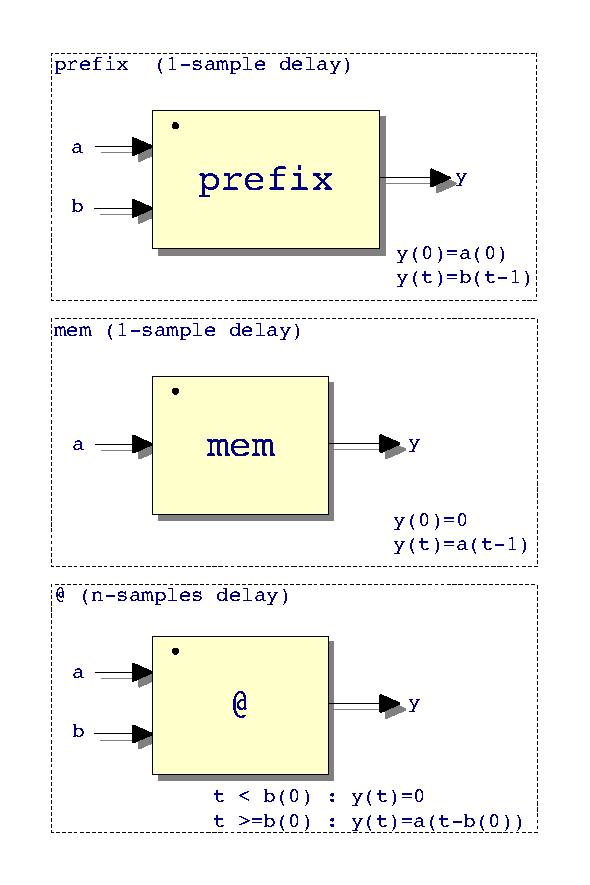
\includegraphics[scale=0.6]{illustrations/faust-diagram4}
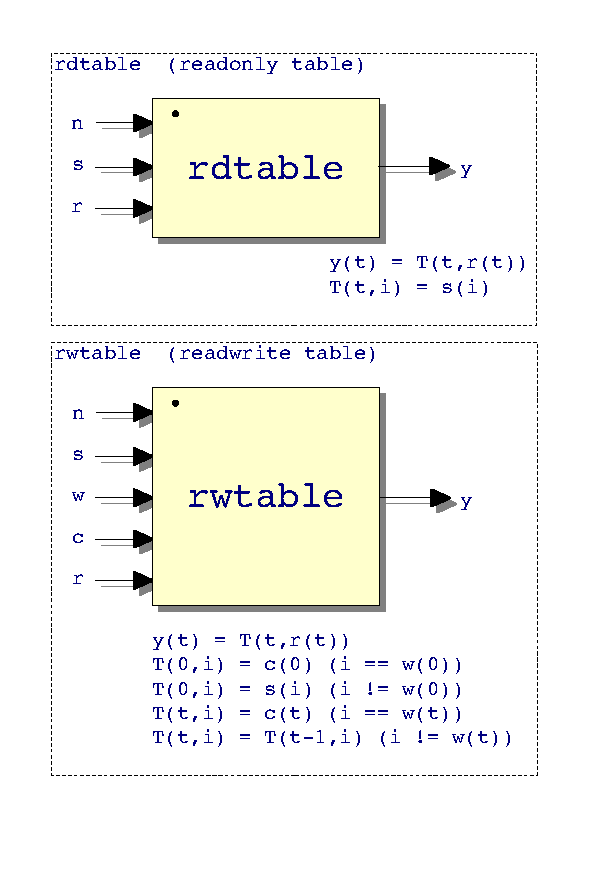
\includegraphics[scale=0.6]{illustrations/faust-diagram5}
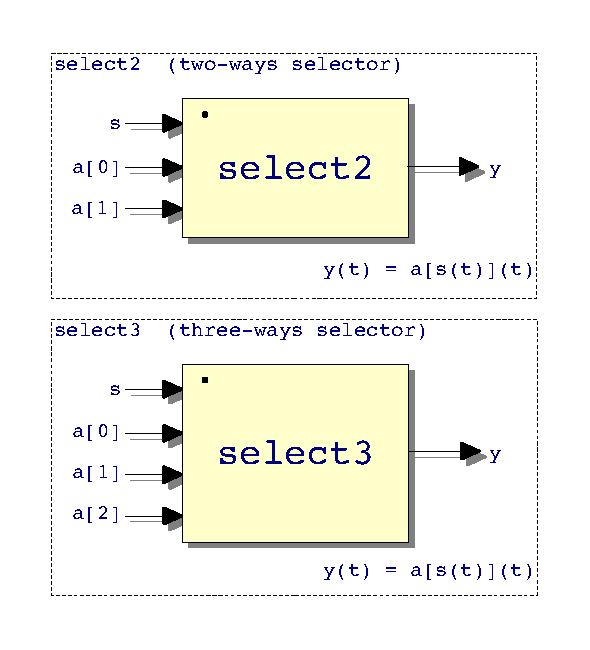
\includegraphics[scale=0.6]{illustrations/faust-diagram6}
\caption{Delays, tables and selectors primitives }
\label{fig:delays}
\end{figure}


%--------------------------------------------------------------------------------------------------------------
\subsection{User Interface Elements}
%--------------------------------------------------------------------------------------------------------------


Faust user interface widgets allow an abstract description of the user interface from within the Faust code. This description is
independent of any GUI toolkits. It is based on \emph{buttons}, \emph{checkboxes}, \emph{sliders}, etc. that are grouped together vertically and
horizontally using appropriate grouping schemes.

All these GUI elements produce signals. A button for example (see figure \ref{fig:button}) produces a signal which is 1 when the button is pressed and 0 otherwise.
These signals can be freely combined with other audio signals.

\begin{figure}[h]
\centering
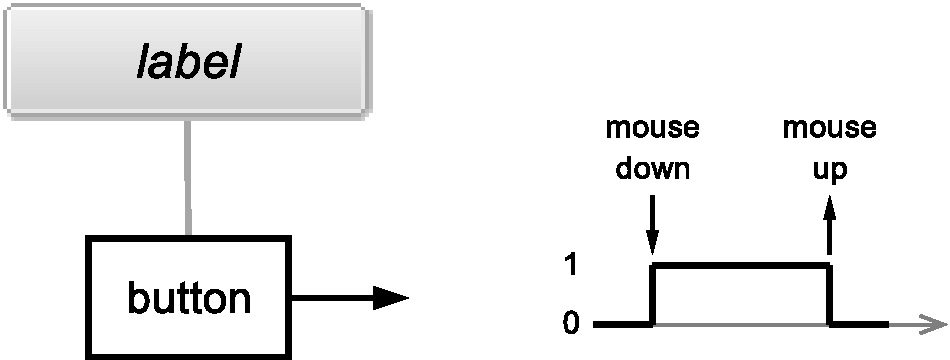
\includegraphics[scale=0.5]{illustrations/button}
\caption{User Interface Button}
\label{fig:button}
\end{figure}


\vspace{5 mm}

\begin{tabular}{|l|l|}
\hline
\textbf{Syntax} & \textbf{Example} \\
\hline
\texttt{button(\farg{str})} & \texttt{button("play")}\\
\texttt{checkbox(\farg{str})} & \texttt{checkbox("mute")}\\
\texttt{vslider(\farg{str},\farg{cur},\farg{min},\farg{max},\farg{step})} & \texttt{vslider("vol",50,0,100,1)}\\
\texttt{hslider(\farg{str},\farg{cur},\farg{min},\farg{max},\farg{step})} & \texttt{hslider("vol",0.5,0,1,0.01)}\\
\texttt{nentry(\farg{str},\farg{cur},\farg{min},\farg{max},\farg{step})} & \texttt{nentry("freq",440,0,8000,1)}\\
\texttt{vgroup(\farg{str},\farg{block-diagram})} & \texttt{vgroup("reverb", \ldots)}\\
\texttt{hgroup(\farg{str},\farg{block-diagram})} & \texttt{hgroup("mixer", \ldots)}\\
\texttt{tgroup(\farg{str},\farg{block-diagram})} & \texttt{vgroup("parametric", \ldots)}\\
\texttt{vbargraph(\farg{str},\farg{min},\farg{max})} & \texttt{vbargraph("input",0,100)}\\
\texttt{hbargraph(\farg{str},\farg{min},\farg{max})} & \texttt{hbargraph("signal",0,1.0)}\\
\hline
\end{tabular}

\vspace{5 mm}

\textbf{note} : The \emph{str} string used in widgets can contain variable parts.
These variable parts are indicated by the sign '\texttt{\%}' followed by the name of a variable.
For example \texttt{par(i,8,hslider("Voice \%i", 0.9, 0, 1, 0.01))} creates 8 different sliders in parallel :
\texttt{hslider("Voice 0", 0.9, 0, 1, 0.01),}
\texttt{hslider("Voice 1", 0.9, 0, 1, 0.01),} \ldots
\texttt{,hslider("Voice 7", 0.9, 0, 1, 0.01)}.

An escape mechanism is provided.
If the sign '\texttt{\%}' is followed by itself, it will be included in the resulting string.
For example \texttt{"feedback (\%\%)"} will result in \texttt{"feedback (\%)"}.



%--------------------------------------------------------------------------------------------------------------
\subsection{The Foreign Function Mechanism}
%--------------------------------------------------------------------------------------------------------------

External C functions, variables and constants can be introduced using the foreign function mechanism.
An external C function is declared by indicating its name and signature as well as the required include file. External variables and constants can also be declared with a similar syntax. 

Variable are considered to vary at block speed. This means that expressions depending of external variables are computed every block, while expressions depending external constants are computed only once at initialization. There is currently no external signals that would be computed every sample. 

The syntax of these foreign declarations is the following :

\begin{rail}
foreign : 'ffunction' '(' signature ',' includefile ',' comment ')' | 'fvariable' '(' type identifier ',' includefile ')' | 'fconstant' '(' type identifier ',' includefile ')' ;
signature : type identifier '(' (type * ',') ')';
type : 'int' | 'float';
\end{rail}


The file \texttt{math.lib} included in the Faust package defines most of the standard mathematical function of
\texttt{<math.h>} (that are not already builtins) using the foreign function mechanism.
Here is the list of these functions :

\vspace{5 mm}

\begin{tabular}{|l|l|}
\hline
\textbf{Name} & \textbf{Definition}   \\
\hline

\texttt{SR 			} & \texttt{ fconstant(int fSamplingFreq, <math.h>)} \\
\texttt{PI 			} & \texttt{ 3.1415926535897932385 } \\
\texttt{cbrt 		} & \texttt{ ffunction(float cbrt (float), <math.h>,"")} \\
\texttt{hypot 		} & \texttt{ ffunction(float hypot (float, float), <math.h>,"")} \\
\texttt{ldexp 		} & \texttt{ ffunction(float ldexp (float, int), <math.h>,"")} \\
\texttt{scalb 		} & \texttt{ ffunction(float scalb (float, float), <math.h>,"")} \\
\texttt{log1p 		} & \texttt{ ffunction(float log1p (float), <math.h>,"")} \\
\texttt{logb 		} & \texttt{ ffunction(float logb (float), <math.h>,"")} \\
\texttt{ilogb 		} & \texttt{ ffunction(int ilogb (float), <math.h>,"")} \\
\texttt{expm1 		} & \texttt{ ffunction(float expm1 (float), <math.h>,"")} \\
\texttt{acosh		} & \texttt{ ffunction(float acosh (float), <math.h>, "")} \\
\texttt{asinh		} & \texttt{ ffunction(float asinh (float), <math.h>, "")} \\
\texttt{atanh		} & \texttt{ ffunction(float atanh (float), <math.h>, "")} \\
\texttt{sinh		} & \texttt{ ffunction(float sinh (float), <math.h>, "")} \\
\texttt{cosh		} & \texttt{ ffunction(float cosh (float), <math.h>, "")} \\
\texttt{tanh		} & \texttt{ ffunction(float tanh (float), <math.h>,"")} \\
\texttt{erf			} & \texttt{ ffunction(float erf(float), <math.h>,"")} \\
\texttt{erfc		} & \texttt{ ffunction(float erfc(float), <math.h>,"")} \\
\texttt{gamma		} & \texttt{ ffunction(float gamma(float), <math.h>,"")} \\
\texttt{J0			} & \texttt{ ffunction(float j0(float), <math.h>,"")} \\
\texttt{J1			} & \texttt{ ffunction(float j1(float), <math.h>,"")} \\
\texttt{Jn			} & \texttt{ ffunction(float jn(int, float), <math.h>,"")} \\
\texttt{lgamma		} & \texttt{ ffunction(float lgamma(float), <math.h>,"")} \\
\texttt{Y0			} & \texttt{ ffunction(float y0(float), <math.h>,"")} \\
\texttt{Y1			} & \texttt{ ffunction(float y1(float), <math.h>,"")} \\
\texttt{Yn			} & \texttt{ ffunction(float yn(int, float), <math.h>,"")} \\
\texttt{isnan 		} & \texttt{ ffunction(int isnan (float),<math.h>,"")} \\
\texttt{nextafter	} & \texttt{ ffunction(float nextafter(float, float),<math.h>,"")} \\
\hline
\end{tabular}

\vspace{5 mm}

%--------------------------------------------------------------------------------------------------------------
\subsection{Programming constructions}
%--------------------------------------------------------------------------------------------------------------

Faust provides several programming constructions that give powerful ways to describe and transform block-diagrams algorithmically.

\begin{rail}
Abstraction :  backslash '(' (ident + ',') ')' '.' '(' blockdiagram ')';
\end{rail} 
\emph{Abstractions} allow to define anonymous functions like for example a square function : $\char"5C (x).(x*x)$. Unapplied abstractions can be used for symbolic routing of signals. For example : $\char"5C (x,y).(y,x)$ denotes a signal processor that exchanges its two inputs. 

\begin{rail}
Case :  "case" lbrace (rule +) rbrace ;
Rule : '(' (pattern + ',') ')' "=>" blockdiagram ';';
Pattern : ident | blockdiagram;
\end{rail}
\emph{case} pattern matching rules provide an effective way to analyze and transform block-diagrams algorithmically. For example \texttt{case\{ (x:y) => y:x; (x) => x; \}} will invert the two parts of a sequential block-diagram and leave untouched any other construction. Please note that patterns are evaluated before the pattern matching operation. Therefore only variables that appear free in the pattern are binding variables during pattern matching. 


\begin{rail}
Component : 'component' '(' filename ')';
\end{rail}
The \emph{component} construction allows a very modular design. A whole Faust program can be included in another Faust program as a simple expression. For example \texttt{component("freeverb.dsp")} denotes the process defined in the file \emph{"freeverb.dsp"}, and 

\begin{tabular}{l}
\texttt{process = component("karplus32.dsp"):component("freeverb.dsp");} \\
\end{tabular}

is a process that combines two components in sequence.

\begin{rail}
par : "par" '(' ident ',' value ',' blockdiagram ')';
seq : "seq" '(' ident ',' value ',' blockdiagram ')';
sum : "sum" '(' ident ',' value ',' blockdiagram ')';
prod : "prod" '(' ident ',' value ',' blockdiagram ')';
\end{rail}
The \texttt{par}, \texttt{seq}, \texttt{sum} and \texttt{prod} constructions allow algorithmic descriptions of block-diagrams.
For example :

\begin{tabular}{lll}
\texttt{par(i,8,E(i))} &is equivalent to &\texttt{E(0),E(1),\ldots ,E(7)} \\
\texttt{seq(i,8,E(i))} &is equivalent to &\texttt{E(0):E(1):\ldots :E(7)} \\
\texttt{sum(i,8,E(i))} &is equivalent to &\texttt{E(0)+E(1)+\ldots +E(7)} \\
\texttt{prod(i,8,E(i))} &is equivalent to &\texttt{E(0)*E(1)*\ldots *E(7)}\\
\end{tabular}


%%%%%%%%%%%%%%%%%%%%%%%%%%%%%%%%%%%%%%%%%%%%%%%%%%%%%%%%%%%%%%%%%%%%%%%%%%%%%%%%%%%%%%
%                            INVOKING THE COMPILER                                             %
%%%%%%%%%%%%%%%%%%%%%%%%%%%%%%%%%%%%%%%%%%%%%%%%%%%%%%%%%%%%%%%%%%%%%%%%%%%%%%%%%%%%%%


\section{Invoking the Faust compiler}
The Faust compiler is invoked using the \texttt{faust} command. It translate Faust programs into C++ code.
The generated code can be wrapped into an optional \emph{architecture file} allowing to directly produce a fully operational program.

\begin{rail}
compiler : "faust" (|options) ( file +);
\end{rail}


Compilation options are listed in the following table :

\vspace{5 mm}

\begin{tabular}{|l|l|l|}
\hline
\textbf{Short} 				& \textbf{long} 					& \textbf{Description}   \\
\hline
\texttt{-h} 				& \texttt{--help} 					& print the help message  \\
\texttt{-v} 				& \texttt{--version} 				& print version information  \\
\texttt{-d} 				& \texttt{--details} 				& print compilation details  \\
\texttt{-ps} 				& \texttt{--postscript} 			& generate block-diagram postscript file  \\
\texttt{-svg} 				& \texttt{--svg} 					& generate block-diagram svg files  \\
\texttt{-f \farg{n}} 		& \texttt{--fold \farg{n}}  		& max complexity of svg diagrams before splitting\\
							&									& into several files (default 25 boxes)  \\
\texttt{-mns \farg{n}} 		& \texttt{--max-name-size \farg{n}} & max character size used in svg diagram labels\\
\texttt{-sn}             	& \texttt{--simple-names}			& use simple names (without arguments) for block-diagram \\
							&									& (default max size : 40 chars) \\
\texttt{-xml} 				& \texttt{--xml} 					& generate an additional description file in xml format  \\
\texttt{-lb}	 			& \texttt{--left-balanced} 			& generate left-balanced expressions  \\
\texttt{-mb} 				& \texttt{--mid-balanced} 			& generate mid-balanced expressions (default)  \\
\texttt{-rb} 				& \texttt{--right-balanced}			& generate right-balanced expressions  \\
\texttt{-mcd \farg{n}}		& \texttt{--max-copy-delay \farg{n}}& threshold between copy and ring buffer delays\\
							&									& (default 16 samples)  \\
\texttt{-a \farg{file}} 	&  									& C++ wrapper file  \\
\texttt{-o \farg{file}} 	&  									& C++ output file  \\
\hline
\end{tabular}

\vspace{5 mm}

The main available architecture files are :

\vspace{5 mm}

\begin{tabular}{|l|l|l|}
\hline
\textbf{File name}			& \textbf{Description}   \\
\hline
\texttt{max-msp.cpp} 		& Max/MSP plugin  \\
\texttt{vst.cpp} 			& VST plugin  \\
\texttt{jack-gtk.cpp} 		& Jack GTK full application  \\
\texttt{jack-qt.cpp} 		& Jack QT full application  \\
\texttt{alsa-gtk.cpp} 		& Alsa GTK full application  \\
\texttt{alsa-qt.cpp} 		& Alsa QT full application  \\
\texttt{oss-gtk.cpp} 		& OSS GTK full application  \\
\texttt{ladspa.cpp} 		& LADSPA plugin  \\
\texttt{q.cpp} 				& Q language plugin  \\
\texttt{supercollider.cpp} 	& SuperCollider Unit Generator  \\
\texttt{sndfile.cpp} 		& sound file transformation command \\
\texttt{bench.cpp} 			& speed benchmark   \\

\hline
\end{tabular}

\vspace{5 mm}

Here is an example of compilation command that generates the C++ source code of a Jack application using the GTK graphic toolkit:

\texttt{faust -a jack-gtk.cpp -o freeverb.cpp freeverb.dsp}.

\vspace{5 mm}

%%%%%%%%%%%%%%%%%%%%%%%%%%%%%%%%%%%%%%%%%%%%%%%%%%%%%%%%%%%%%%%%%%%%%%%%%%%%%%%%%%%%%%
%%%%%%%%%%%%%%%%%%%%%%%%%%%%%%%%%%%%%%%%%%%%%%%%%%%%%%%%%%%%%%%%%%%%%%%%%%%%%%%%%%%%%%
%                            		END                                              %
%%%%%%%%%%%%%%%%%%%%%%%%%%%%%%%%%%%%%%%%%%%%%%%%%%%%%%%%%%%%%%%%%%%%%%%%%%%%%%%%%%%%%%
%%%%%%%%%%%%%%%%%%%%%%%%%%%%%%%%%%%%%%%%%%%%%%%%%%%%%%%%%%%%%%%%%%%%%%%%%%%%%%%%%%%%%%


\end{document}
